\documentclass[hyperref, a4paper]{article}

\usepackage{geometry}
\usepackage{titling}
\usepackage{titlesec}
% No longer needed, since we will use enumitem package
% \usepackage{paralist}
\usepackage{enumitem}
\usepackage{footnote}
\usepackage[colorinlistoftodos]{todonotes}
\usepackage{amsmath, amssymb, amsthm}
\usepackage{mathtools}
\usepackage{bbm}
\usepackage{graphicx}
\usepackage{subcaption}
\usepackage{soulutf8}
\usepackage{physics}
\usepackage{tensor}
\usepackage{siunitx}
\usepackage[version=4]{mhchem}
\usepackage{tikz}
\usepackage{xcolor}
\usepackage{listings}
\usepackage{autobreak}
\usepackage[ruled, vlined, linesnumbered]{algorithm2e}
\usepackage{nameref,zref-xr}
\zxrsetup{toltxlabel}
\usepackage[backend=bibtex]{biblatex}
\addbibresource{elasticity.bib}
\usepackage[colorlinks,unicode]{hyperref} % , linkcolor=black, anchorcolor=black, citecolor=black, urlcolor=black, filecolor=black
\usepackage[most]{tcolorbox}
\usepackage{prettyref}

% Page style
\geometry{left=3.18cm,right=3.18cm,top=2.54cm,bottom=2.54cm}
\titlespacing{\paragraph}{0pt}{1pt}{10pt}[20pt]
\setlength{\droptitle}{-5em}

% More compact lists 
\setlist[itemize]{
    itemindent=17pt, 
    leftmargin=1pt,
    listparindent=\parindent,
    parsep=0pt,
}

% Math operators
\DeclareMathOperator{\timeorder}{\mathcal{T}}
\DeclareMathOperator{\diag}{diag}
\DeclareMathOperator{\legpoly}{P}
\DeclareMathOperator{\primevalue}{P}
\DeclareMathOperator{\sgn}{sgn}
\DeclareMathOperator{\res}{Res}
\DeclareMathOperator{\sinc}{sinc}
\newcommand*{\ii}{\mathrm{i}}
\newcommand*{\ee}{\mathrm{e}}
\newcommand*{\const}{\mathrm{const}}
\newcommand*{\suchthat}{\quad \text{s.t.} \quad}
\newcommand*{\argmin}{\arg\min}
\newcommand*{\argmax}{\arg\max}
\newcommand*{\normalorder}[1]{: #1 :}
\newcommand*{\pair}[1]{\langle #1 \rangle}
\newcommand*{\fd}[1]{\mathcal{D} #1}
\DeclareMathOperator{\bigO}{\mathcal{O}}

% TikZ setting
\usetikzlibrary{arrows,shapes,positioning}
\usetikzlibrary{arrows.meta}
\usetikzlibrary{decorations.markings}
\usetikzlibrary{calc}
\tikzstyle arrowstyle=[scale=1]
\tikzstyle directed=[postaction={decorate,decoration={markings,
    mark=at position .5 with {\arrow[arrowstyle]{stealth}}}}]
\tikzstyle ray=[directed, thick]
\tikzstyle dot=[anchor=base,fill,circle,inner sep=1pt]

% Algorithm setting
% Julia-style code
\SetKwIF{If}{ElseIf}{Else}{if}{}{elseif}{else}{end}
\SetKwFor{For}{for}{}{end}
\SetKwFor{While}{while}{}{end}
\SetKwProg{Function}{function}{}{end}
\SetArgSty{textnormal}

\newcommand*{\concept}[1]{{\textbf{#1}}}

% Embedded codes
\lstset{basicstyle=\ttfamily,
  showstringspaces=false,
  commentstyle=\color{gray},
  keywordstyle=\color{blue}
}

% Reference formatting
\newcommand*{\citesec}[1]{\S~{#1}}
\newcommand*{\citechap}[1]{chap.~{#1}}
\newcommand*{\citefig}[1]{Fig.~{#1}}
\newcommand*{\citetable}[1]{Table~{#1}}
\newcommand*{\citepage}[1]{pp.~{#1}}
\newrefformat{fig}{Fig.~\ref{#1}}
\newcommand*{\term}[1]{\textit{#1}}

% Color boxes
\tcbuselibrary{skins, breakable, theorems}

\newtcbtheorem{infobox}{Box}{
    enhanced,
    boxrule=0pt,
    colback=blue!5,
    colframe=blue!5,
    coltitle=blue!50,
    borderline west={4pt}{0pt}{blue!65},
    sharp corners,
    fonttitle=\bfseries, 
    breakable,
    before upper={\parindent15pt\noindent}}{box}
\newtcbtheorem[use counter from=infobox]{theorybox}{Box}{
    enhanced,
    boxrule=0pt,
    colback=orange!5, 
    colframe=orange!5, 
    coltitle=orange!50,
    borderline west={4pt}{0pt}{orange!65},
    sharp corners,
    fonttitle=\bfseries, 
    breakable,
    before upper={\parindent15pt\noindent}}{box}
\newtcbtheorem[use counter from=infobox]{learnbox}{Box}{
    enhanced,
    boxrule=0pt,
    colback=green!5,
    colframe=green!5,
    coltitle=green!50,
    borderline west={4pt}{0pt}{green!65},
    sharp corners,
    fonttitle=\bfseries, 
    breakable,
    before upper={\parindent15pt\noindent}}{box}


\newenvironment{shelldisplay}{\begin{lstlisting}}{\end{lstlisting}}

\newcommand*{\kB}{k_{\text{B}}}
\newcommand*{\muB}{\mu_{\text{B}}}
\newcommand*{\efermi}{E_{\text{F}}}
\newcommand*{\pfermi}{p_{\text{F}}}
\newcommand*{\vfermi}{v_{\text{F}}}
\newcommand*{\sA}{\text{A}}
\newcommand*{\sB}{\text{B}}
\newcommand*{\Tc}{T_{\text{c}}}
\newcommand*{\hethree}{$^3$He}
\newcommand*{\hefour}{$^4$He}
\newcommand{\epsr}{\epsilon_{\text{r}}}
\newcommand*{\mur}{\mu_{\text{r}}}
\newcommand{\chie}{\chi_{\text{e}}}
\newcommand*{\Gammae}{\Gamma_{\text{e}}}
\newcommand*{\Gammag}{\Gamma_{\text{g}}}
\newcommand*{\omegae}{\omega_{\text{e}}}
\newcommand*{\omegag}{\omega_{\text{g}}}
\newcommand*{\omegaeg}{\omega_{\text{eg}}}
\newcommand*{\ptwfc}[2]{\psi^{(#2)}_{#1}}
\newcommand*{\mueg}{\mu_{\text{eg}}}
\newcommand*{\muge}{\mu_{\text{ge}}}
\newcommand*{\Ezzero}{E_{z0}}
\newcommand*{\kete}{\ket*{\text{e}}}
\newcommand*{\ketg}{\ket*{\text{g}}}
\newcommand*{\coeffe}{c_{\text{e}}}
\newcommand*{\coeffg}{c_{\text{g}}}
\newcommand*{\pope}{p_{\text{e}}}
\newcommand*{\popg}{p_{\text{g}}}
\newcommand*{\ptwo}{P^{(2)}}
\newcommand*{\vp}{v_{\text{p}}}
\newcommand*{\chitwo}{\chi^{(2)}}
\newcommand*{\chithree}{\chi^{(3)}}
\newcommand*{\omegap}{\omega_{\text{p}}}
\newcommand*{\mvb}[1]{\tilde{\vb*{#1}}}
\newcommand*{\Si}[1]{S_{\text{i#1}}}
\newcommand*{\So}[1]{S_{\text{o#1}}}
\newcommand*{\taug}{\tau_{\text{g}}}

\title{Homework 3}
\author{Jinyuan Wu}

\begin{document}

\maketitle

\section{}

\subsection{}

\textit{Asymmetric Fabry-Perot resonator: In this problem, we use coupled mode theory to approximate the response of a generalized Fabry-Perot resonator. For example, this system could be a photonic crystal defect coupled to two defect waveguide (see Figure 4 in Ch 10 of [JJSJ]) or it could be a conventional a two-mirror Fabry-Perot; the underlying physics is strikingly similar. To formulate the response, we consider a single mode, $a$, that is coupled to input/output ports, seen in Fig. 1(a). To account for the fact that the two mirrors of the system can have different reflectivities, Ports 1 and Port 2 have distinct coupling strengths $\kappa_1=\sqrt{2 / \tau_1}$ and $\kappa_2=\sqrt{2 / \tau_2}$. We begin our analysis of this system by assuming that our mode has no intrinsic damping (i.e., the only pathway modal energy loss comes from the coupling rates $\kappa_1$ and $\kappa_2$ ), and we analyze the response the system to incident wave amplitude $S_i^1$ entering through Port 1.
}

\paragraph*{(a)} \textit{Find an expression for the frequency dependent reflectivity of Port $1,\left(S_o^1 / S_i^1\right)$ and the transmissivity from Port 1 to Port $2,\left(S_o^2 / S_i^1\right)$. Show that this system conserves power.} 

Since $\kappa_1$ and $\kappa_2$ both contain no phase factors, 
we can set $\alpha_1 = \alpha_2 = 0$.
The EOMs are 
\begin{equation}
    \dot{a} = - \ii \omega_0 a - \left(\frac{1}{\tau_1} + \frac{1}{\tau_2}\right) a + 
    \kappa_1 \Si{1} + \kappa_2 \Si{2}, \quad 
    \So{1,2} = - \Si{1,2} + \sqrt{\frac{2}{\tau_{1,2}}} a.
\end{equation}
Considering the Fourier component with frequency $\omega$, we find 
\[
    - \ii \omega a(\omega) = - \ii \omega_0 a(\omega) - \left(\frac{1}{\tau_1} + \frac{1}{\tau_2}\right) a(\omega) + 
    \kappa_1 \Si{1}(\omega) + \kappa_2 \Si{2}(\omega),
\]
and hence by eliminating $a(\omega)$ and setting $\Si{2} = 0$, we find 
\begin{equation}
    \frac{\So{1}}{\Si{1}} = \frac{2}{\tau_1} \frac{1}{- \ii \omega + \ii \omega_0 + \frac{1}{\tau_1} + \frac{1}{\tau_2}} - 1,
\end{equation}
\begin{equation}
    \frac{\So{2}}{\Si{1}} = \frac{2}{\sqrt{\tau_1 \tau_2}} \frac{1}{- \ii \omega + \ii \omega_0 + \frac{1}{\tau_1} + \frac{1}{\tau_2}}.
\end{equation}
It can be straightforwardly demonstrated that 
\begin{equation}
    \abs{\frac{\So{1}}{\Si{1}}}^2 + \abs{\frac{\So{2}}{\Si{1}}}^2 = 1
\end{equation}
and therefore we have energy conservation.

\paragraph*{(b)} \textit{Under what conditions do we have lossless resonant transmission from Port 1 to Port 2. This condition is commonly referred to as 'critical coupling'.} 

What we want is that $\abs*{\So{2} / \Si{1}}^2 = 1$, which is equivalent to 
\[
    \frac{4}{\tau_1 \tau_2} \frac{1}{(\omega - \omega_0)^2 + \left( \frac{1}{\tau_1} + \frac{1}{\tau_2} \right)^2} = 1,
\]
which reduces to 
\[
    (\omega_0 - \omega)^2 + \left( \frac{1}{\tau_1} - \frac{1}{\tau_2} \right)^2 = 0,
\]
and hence is equivalent to
\begin{equation}
    \omega = \omega_0, \quad \tau_1 = \tau_2. 
\end{equation}

\paragraph*{(c)} \textit{Next, the we assume that our mode has an internal decay rate, $1 / \tau_o$. Can the transmission reach unity? What conditions must be satisfied for the reflectivity from port 1 to vanish? Is the fractional energy absorption necessarily the same for waves entering Port 1 and Port 2 (Explain)?} 

In this case, the EOM of $a$ in the frequency domain is
\begin{equation}
    - \ii \omega a(\omega) = - \ii \omega_0 a(\omega) - \left(\frac{1}{\tau_0} + \frac{1}{\tau_1} + \frac{1}{\tau_2}\right) a(\omega) + 
    \kappa_1 \Si{1}(\omega) + \kappa_2 \Si{2}(\omega),
\end{equation}
and repeating the above procedure we find the transmission from port 1 to port 2 is 
\begin{equation}
    \frac{\So{2}}{\Si{1}} = \frac{2}{\sqrt{\tau_1 \tau_2}} \frac{1}{- \ii \omega + \ii \omega_0 + \frac{1}{\tau_0} + \frac{1}{\tau_1} + \frac{1}{\tau_2}}.
\end{equation}
The condition that $\abs*{\So{2} / \Si{1}} = 1$ is equivalent to 
\[
    \frac{4}{\tau_1 \tau_2} \frac{1}{(\omega - \omega_0)^2 + \left( \frac{1}{\tau_0} + \frac{1}{\tau_1} + \frac{1}{\tau_2} \right)^2} = 1,
\]
which is equivalent to 
\begin{equation}
    (\omega - \omega_0)^2 + \left( \frac{1}{\tau_1} - \frac{1}{\tau_2} \right)^2 
    + \frac{1}{\tau_0^2} + \frac{2}{\tau_0} \left( \frac{1}{\tau_1} + \frac{1}{\tau_2} \right) = 0.
\end{equation}
Since the square terms are either zero or greater than zero,
and the $1/\tau_0$ terms are strictly greater than zero, 
this equation can't be satisfied, 
and therefore the transmission can never reach unity.

On the other hand, letting the reflectivity from port 1 to vanish is possible.
What we want is for
\begin{equation}
    \frac{\So{1}}{\Si{1}} = \frac{2}{\tau_1} \frac{1}{- \ii \omega + \ii \omega_0 + \frac{1}{\tau_0} + \frac{1}{\tau_1} + \frac{1}{\tau_2}} - 1
\end{equation}
to be zero, which is equivalent to 
\[
    \ii (\omega_0 - \omega) + \frac{1}{\tau_0} + \frac{1}{\tau_2} - \frac{1}{\tau_1} = 0,
\] 
and therefore the condition of zero reflectivity at port 1 is 
\begin{equation}
    \omega = \omega_0, \quad \frac{1}{\tau_0} + \frac{1}{\tau_2} = \frac{1}{\tau_1}.
\end{equation}

\paragraph*{(d)} \textit{Next, we add optical amplification to our dissipative system from Part (c); we also assume that both mirrors have identical reflectivity (i.e., $\kappa_1=\kappa_2$ ). In the small signal limit (i.e., neglecting saturation of the gain mechanism), we can include the effects of optical amplification by adding an effective gain rate (or a negative decay rate) of $1 / \tau_g$. Under what conditions does the transmission reach unity? Under what conditions does the the resonantly transmitted power become amplified? Identify the conditions for self-oscillation?} 

Replacing $1/\tau_0$ by $1 / \tau_0 - 1/\taug$, and defining $\tau \coloneqq \tau_1 = \tau_2$, we have 
\begin{equation}
    \frac{\So{2}}{\Si{1}} = \frac{2}{\sqrt{\tau_1 \tau_2}} 
    \frac{1}{- \ii \omega + \ii \omega_0 
    + \frac{1}{\tau_0} - \frac{1}{\taug} + \frac{1}{\tau_1} + \frac{1}{\tau_2}}.
\end{equation}

For the transmission to reach unity, we need to have
\[
    (\omega - \omega_0)^2 + \left( \frac{1}{\tau_0} - \frac{1}{\taug} + \frac{1}{\tau_1} + \frac{1}{\tau_2} \right)^2
    = \frac{4}{\tau_1 \tau_2},
\]
or equivalently 
\begin{equation}
    (\omega - \omega_0)^2 + \left( \frac{1}{\tau_1} - \frac{1}{\tau_2} \right)^2 
    + \left( \frac{1}{\tau_0} - \frac{1}{\taug} \right)^2 + 2 \left( \frac{1}{\tau_0} - \frac{1}{\taug} \right) \left( \frac{1}{\tau_1} + \frac{1}{\tau_2} \right) = 0.
\end{equation}
Unlike the case with $1 / \tau_0$ only, 
here the fourth term can be negative because $\taug$ can be arbitrarily small.
If $\frac{1}{\tau_0} - \frac{1}{\taug}$ is regarded as the unknown value,
the equation has real solutions if and only if 
\begin{equation}
    \frac{4}{\tau_1 \tau_2} \geq (\omega - \omega_0)^2. 
\end{equation}
When this condition is not satisfied, 
it's impossible for the transmission to reach unity; 
when it is satisfied, 
the transmission reaches unity when 
\begin{equation}
    \frac{1}{\taug} = \frac{1}{\tau_0} + \frac{1}{\tau_1} + \frac{1}{\tau_2} 
    \pm \sqrt{
        \frac{4}{\tau_1 \tau_2} - (\omega - \omega_0)^2
    }.
\end{equation}
When the transmitted power is amplified, we have $\abs{\frac{\So{2}}{\Si{1}}}^2 \geq 1$, 
which is equivalent to 
\begin{equation}
    \frac{1}{\tau_0} + \frac{1}{\tau_1} + \frac{1}{\tau_2} 
    - \sqrt{
        \frac{4}{\tau_1 \tau_2} - (\omega - \omega_0)^2
    } 
    \leq \frac{1}{\taug} \leq \frac{1}{\tau_0} + \frac{1}{\tau_1} + \frac{1}{\tau_2} 
    + \sqrt{
        \frac{4}{\tau_1 \tau_2} - (\omega - \omega_0)^2
    }.
\end{equation} 

Self-oscillation means emergence of oscillation even when there is no driving, 
which is equivalent to an infinite response function.
Therefore it appears when 
\begin{equation}
    \omega = \omega_0, \quad \frac{1}{\taug} = \frac{1}{\tau_0} + \frac{1}{\tau_1} + \frac{1}{\tau_2}.
\end{equation}

\subsection{}

\textit{Fano resonance: In this problem we consider a mode with two ports, as in problem 1.1, but now the ports are also directly coupled to each other, as illustrated in Fig. 1c. This gives rise to a transmission/reflection profile which is not symmetric around the central resonant frequency. This phenomenon is observed in many systems, for example in conventional atomic spectroscopy.}

\paragraph*{(a)} \textit{Suppose there is no input wave but the mode starts with some energy. Use energy conservation (like in L13.N1) and the given equations to show that $\tau^{-1}=\left(\left|\kappa_1\right|^2+\left|\kappa_2\right|^2\right) / 2=|\kappa|^2 / 2$.} 

The EOMs are
\begin{equation}
    \dot{a} = \left( - \ii \omega_0 - \frac{1}{\tau} \right) a 
    + \underbrace{\sum_{l=1}^{2} \kappa^l \Si{}^l}_{\vb{\kappa}^\top \vb{\Si{}}}, 
\end{equation}
\begin{equation}
    \So{}^j = \sum_{l=1}^{2} C_{jl} \Si{}^l + \kappa_j a, \quad 
    \vb{\So{}} = \vb{C} \vb{\Si{}} + a \vb{\kappa}.
\end{equation}
When the input wave is turned off, we have 
\begin{equation}
    \dot{a} = \left( - \ii \omega_0 - \frac{1}{\tau} \right) a,
\end{equation}
and the decay of the energy $U = \abs*{a}^2$ stored in $a$ is given by 
\begin{equation}
    \dv{U}{t} = a^* \dot{a} + \text{c.c.}
    = - \frac{2}{\tau} a^* a = - \frac{2}{\tau} U.
\end{equation}
The energy loss of $a$ comes from the energy gain of $\So{}^{1,2}$, so we expect to see 
\begin{equation}
    - \dv{U}{t} = \sum_l \abs*{\So{}^l}^2 = (\abs*{\kappa_1}^2 + \abs*{\kappa_2}^2) \abs*{a}^2, 
\end{equation}
and therefore 
\begin{equation}
    \frac{2}{\tau} = \abs*{\kappa_1}^2 + \abs*{\kappa_2}^2
    = \vb{\kappa}^\dagger \vb{\kappa} .
\end{equation}

\paragraph*{(b)} \textit{Now we find constraints on the port coupling matrix $C$. In the previous part, we used the fact that the output from port $j$ is $S_o^j=\kappa_j a$ in absence of input. Use time-reversal symmetry to show $C \kappa^*=-\kappa$. [Hint: review how we found $\beta=-1$ in L13.N3] $\kappa^*$ is the complex conjugate of $\kappa$, not the conjugate transpose.} 

Applying time reversal operation to $\vb{\So{}} = \vb{C} \vb{\Si{}} + a \vb{\kappa}$, we get 
\[
    \vb{\Si{}}^*(-t) = \vb{C} \vb{\So{}}^*(-t) + a^*(-t) \vb{\kappa},
\]
\begin{equation}
    \vb{\Si{}} = \vb{C}^* \vb{\So{}} + a \vb{\kappa}^*.
\end{equation}
The two equations have to be equivalent to each other, 
and therefore when the input wave is turned off, we have 
\[ 
    \vb{C}^* a \kappa + a \kappa^* = 0,
\]
and therefore
\begin{equation}
    \vb{C} \vb{\kappa}^* = - \vb{\kappa}.
\end{equation}
If we instead focus on $\vb{\Si{}}$ terms, we will find 
\begin{equation}
    \vb{C} \vb{C}^* = 1.
\end{equation}

\paragraph*{(c)} Find the $2 \times 2$ frequency-dependent scattering matrix $\sigma[\omega]$, defined by $S_o[\omega]=\sigma[\omega] S_i[\omega]$, in terms of $\tau, \kappa$, and $C$.

Switching to the frequency domain, we have 
\[
    a(\omega) = \frac{1}{- \ii \omega + \ii \omega_0 + \frac{1}{\tau}} \vb{\kappa}^\top \vb{\Si{}}(\omega),
\]
and therefore 
\[
    \vb{\So{}}(\omega) = \vb{C} \vb{\Si{}} + \vb{\kappa} a 
    = \left(
        \vb{C} + \frac{1}{- \ii \omega + \ii \omega_0 + \frac{1}{\tau}} \vb{\kappa} \vb{\kappa}^\top 
    \right) \vb{\Si{}} ,
\]
\begin{equation}
    \vb{\sigma}(\omega) = \vb{C} + \frac{1}{- \ii \omega + \ii \omega_0 + \frac{1}{\tau}} \vb{\kappa} \vb{\kappa}^\top .
\end{equation}

\paragraph*{(d)} \textit{Using the fact that $C$ is unitary and the relation you found in part (c), show that the scattering matrix $\sigma[\omega]$ is unitary.} 

$\vb{C}$ has to be unitary so we have energy conservation 
when the coupling between the mode and the ports is weak.
On the other hand it has been proved that because of time reversal symmetry, 
$\vb{C} \vb{C}^* = 1$.
We therefore find 
\begin{equation}
    \vb{C}^\dagger = \vb{C}^*, \quad \vb{C} = \vb{C}^\top.
\end{equation}
From $\vb{C} \vb{\kappa}^* = - \vb{\kappa}$ we also have 
\begin{equation}
    - \vb{\kappa}^* = \vb{C}^* \vb{\kappa} = \vb{C}^\dagger \vb{\kappa}, \quad 
    \vb{\kappa}^\top \vb{C}^* = - \vb{\kappa}^\dagger, \quad 
    \vb{\kappa}^\dagger \vb{C} = - \vb{\kappa}^\top.
\end{equation}
Therefore 
\begin{equation}
    \begin{aligned}
        \vb{\sigma}^\dagger(\omega) \vb{\sigma}(\omega) &= \vb{C}^\dagger \vb{C} 
        + \vb{C}^\dagger \frac{1}{- \ii \omega + \ii \omega_0 + \frac{1}{\tau}} \vb{\kappa} \vb{\kappa}^\top 
        +  \frac{1}{\ii \omega - \ii \omega_0 + \frac{1}{\tau}} \vb{\kappa}^* \vb{\kappa}^\dagger \vb{C} 
        + \frac{\kappa^* \kappa^\dagger \kappa \kappa^\top}{(\omega - \omega_0)^2 + \frac{1}{\tau^2}} \\
        &= 1 - \frac{\kappa^* \kappa^\top}{- \ii \omega + \ii \omega_0 + \frac{1}{\tau}}
        - \frac{\kappa^* \kappa^\top}{\ii \omega - \ii \omega_0 + \frac{1}{\tau}}
        + \frac{2}{\tau} \frac{\vb{\kappa}^* \vb{\kappa}^\top}{(\omega - \omega_0)^2 + \frac{1}{\tau^2}} \\
        &= 1,
    \end{aligned}
\end{equation}
and therefore $\vb{\sigma}$ is unitary.

\paragraph*{(e)} \textit{Find the overall reflection coefficient $R[\omega]=\left|\sigma_{11}\right|^2$.} 

\begin{equation}
    \sigma_{11} = C_{11} + \frac{1}{- \ii \omega + \ii \omega_0 + \frac{1}{\tau}} \kappa_1^2,
\end{equation}
and therefore 
\begin{equation}
    R(\omega) = \abs*{C_{11}}^2 + \frac{\abs*{\kappa_1}^4}{(\omega - \omega_0)^2 + \frac{1}{\tau^2}} 
    + 2\Re \frac{ C_{11}^* \kappa_1^2}{- \ii \omega + \ii \omega_0 + \frac{1}{\tau}} .
\end{equation}

\textit{From here on, we set $C=\left[\begin{array}{cc}r & -i t \\ -i t & r\end{array}\right]$, where $r$ and $t$ are real and $r^2+t^2=1$.}

\paragraph*{(f)} \textit{Show that $\kappa=\left[\begin{array}{ll}\kappa_1 & \kappa_1\end{array}\right]^T$ can satisfy $C \kappa^*=-\kappa$ with $C$ given above. Define phases $\theta$ and $\phi$ by $r-i t=e^{i \theta}$ and $\kappa_1=\left|\kappa_1\right| e^{i \phi}$. How must $\phi$ be related to $\theta$ to satisfy the equation?} 
    
The equation $\vb{C} \vb{\kappa}^* = - \vb{\kappa}$ reduces to 
\begin{equation}
    r \kappa_1^* - \ii t \kappa_1^* = - \kappa_1.
\end{equation}
This is equivalent to 
\[
    \ee^{\ii \theta} \abs*{\kappa_1} \ee^{- \ii \phi} = - \abs*{\kappa_1} \ee^{\ii \phi},
\] 
and therefore 
\begin{equation}
    \theta - 2 \phi = \pi + 2 \pi n, 
\end{equation}
where $n$ is an integer.

\paragraph*{(g)} \textit{Continuing from the previous part, assume $r \leq 0$ and $t \geq 0$ and use $\phi=(\theta-\pi) / 2$ to express $\kappa_1$ in terms of $r, t$, and $\tau$. [Hint: you will need to use half-angle formulas.]} 

The amplitude of 
\begin{equation}
    \kappa_1 = \abs*{\kappa_1} \ee^{\ii \phi}
\end{equation}
is given by 
\[
    \frac{1}{\tau} = \abs*{\kappa_1}^2, 
\]
while the phase is given by 
\begin{equation}
    \phi = \frac{\theta - \pi}{2}, \quad 
    r - \ii t = \ee^{\ii \theta}.
\end{equation}
Therefore 
\begin{equation}
    \ee^{\ii \phi} = - \ii \ee^{\ii \theta / 2}
    = - \ii \sqrt{r - \ii t}.
\end{equation}
Since $\pi \leq \theta \leq 3\pi /2 $ (because $r \leq 0, t \geq 0$),
$\sin \phi \geq 0, \cos \phi \geq 0$.
The expression of $\kappa_1$ then is 
\begin{equation}
    \kappa_1 = - \frac{\ii}{\sqrt{\tau}} \sqrt{r - \ii t}.
\end{equation}

\paragraph*{(h)} \textit{Finally, combine your results from part (f) and (h) to show
$$
R=\frac{r^2\left(\omega-\omega_0\right)^2+t^2 / \tau^2-2 r t\left(\omega-\omega_0\right) / \tau}{1 / \tau^2+\left(\omega-\omega_0\right)^2} .
$$
}

\textit{Identify which term in the expression gives rise to asymmetry. Plot $R[\omega]$ around the resonant frequency for several values of $\{r, t\}$.}

\begin{equation}
    \begin{aligned}
        R &= r^2 + \frac{\abs*{\kappa_1}^4}{(\omega - \omega_0)^2 + \frac{1}{\tau^2}}
        - \frac{2 r}{\tau} \Re \frac{r - \ii t}{- \ii \omega + \ii \omega_0 + \frac{1}{\tau}} \\
        &= r^2 + \frac{\frac{1}{\tau^2}}{(\omega - \omega_0)^2 + \frac{1}{\tau^2}}
        - \frac{2 r}{\tau} \frac{\frac{r}{\tau} + t (\omega - \omega_0)}{(\omega - \omega_0)^2 + \frac{1}{\tau^2}} \\
        &= \frac{r^2 (\omega - \omega_0)^2 + \frac{t^2}{\tau^2} - \frac{2 r t}{\tau} (\omega - \omega_0)}{(\omega - \omega_0)^2 + \frac{1}{\tau^2}}.
    \end{aligned}
\end{equation}
What makes the shape of the $R$-$\omega$ curve asymmetric is the $- 2 r t (\omega - \omega_0)$ term, 
which comes from the $- \ii t$ term in the first line, 
which in turn comes from the non-diagonal components of $\vb{C}$.
\prettyref{fig:r-plot} shows some $R(\omega)$ curves with different $r$'s.

\begin{figure}
    \centering
    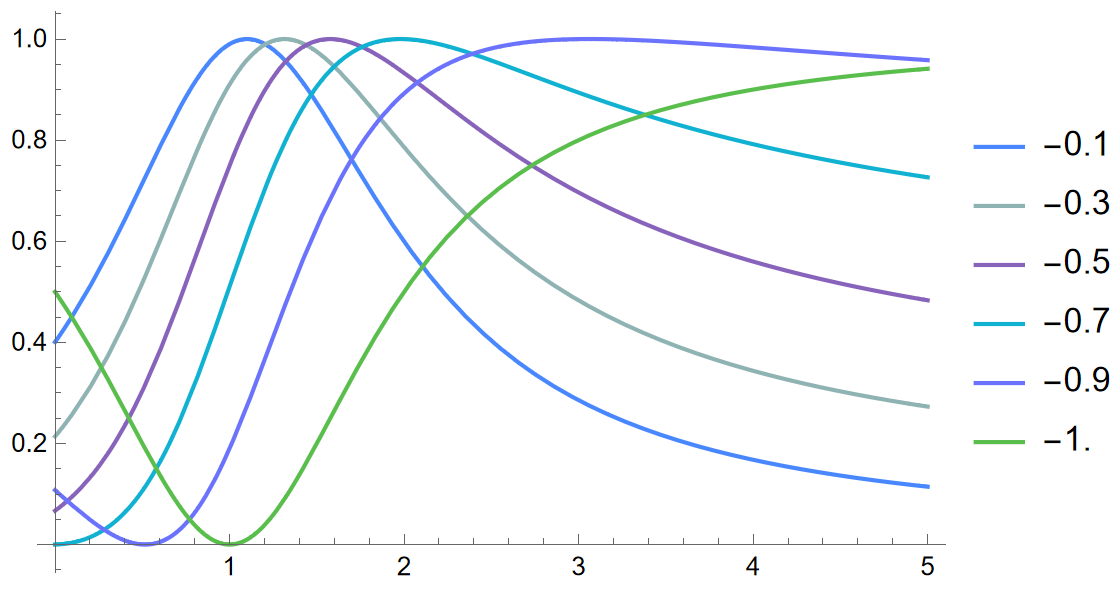
\includegraphics[width=0.5\textwidth]{figs/homework-3-R.png}
    \caption{Plots of $R(\omega)$ with different $t$; the $x$ axis is $\omega / \tau$, 
    and we have chosen $\omega_0 = \tau$.}
    \label{fig:r-plot}
\end{figure}

\section{}

\textit{Background: We can express the response of a physical system using either a scattering $(S)$ matrix or a transfer matrix $(M)$; these different matrix representations relate the input and output waves of a two-port system according to the convention shown below.
}
\begin{center}
    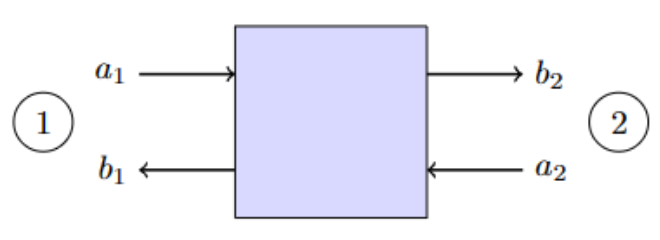
\includegraphics[width=0.4\textwidth]{figs/two-port.PNG}
\end{center}
$$
\left(\begin{array}{l}
b_1 \\
b_2
\end{array}\right)=\left(\begin{array}{ll}
S_{11} & S_{12} \\
S_{21} & S_{22}
\end{array}\right)\left(\begin{array}{l}
a_1 \\
a_2
\end{array}\right), \quad\left(\begin{array}{l}
b_2 \\
a_2
\end{array}\right)=\left(\begin{array}{ll}
M_{11} & M_{12} \\
M_{21} & M_{22}
\end{array}\right)\left(\begin{array}{l}
a_1 \\
b_1
\end{array}\right)
$$
\textit{Throughout, we normalize the input $\left(a_k\right)$ and output $\left(b_k\right)$ wave amplitudes such that the power entering (exiting) the $k^{\text {th }}$ port is given by $\left|a_k\right|^2\left(\left|b_k\right|^2\right)$. Note that the $S$-matrix $\left(S_{i j}\right)$ returns the outgoing wave amplitudes $\left(b_1, b_2\right)$ given the in-going amplitudes $\left(a_1, a_2\right)$. By comparison, the transfer matrix $\left(M_{i j}\right)$ relates both in- and out-going amplitudes at Port $1\left(a_1, b_1\right)$ to the in- and out-going amplitudes at Port $2\left(a_2, b_2\right)$.
}

\subsection{}

\paragraph*{(a)} \textit{Show that a lossless system, where the total power flowing in equals to the power coming out, will result in a unitary $S$-matrix.} 

Since the power going into the system has to be the same as the power going out of the system, we have 
\[
    \sum_i \abs*{b_i}^2 = \sum_i \abs*{a_i}^2, 
\]
and therefore 
\[
    \vb{a}^\dagger \vb{S}^\dagger \vb{S} \vb{a} = \vb{a}^\dagger \vb{a}
\]
for all possible $\vb{a}$ configurations, and therefore 
\begin{equation}
    \vb{S}^\dagger \vb{S} = I 
\end{equation}
and $\vb{S}$ is unitary.

\paragraph*{(b)} \textit{When examining the time reversed response of the system, the waves flip their propagation direction (i.e. inputs become outputs) and are complex conjugated. Show how this results in the $S$-matrix satisfying $S^*=S^{-1}$.} 

Applying the time reversal operation to $\vb{b} = \vb{S} \vb{a}$, we have 
\[
    \vb{a}^* = \vb{S} \vb{b}^*,
\]
where all $a$ operators become $\vb{b}$ operators 
because under the time reversal operation the direction of mode propagation is swapped, 
and hence the mode labels are swapped, 
and since the operators are complex, 
a complex conjugate operation is also applied.
Now if the system has time reversal symmetry, 
$\vb{a}^* = \vb{S} \vb{b}^*$ and $\vb{b} = \vb{S} \vb{a}$ should both be true, 
and therefore for every possible configuration of $\vb{b}$, 
\[
    \vb{b} = \vb{S} \vb{S}^* \vb{b},
\] 
and therefore 
\begin{equation}
    \vb{S} \vb{S}^* = I , \quad \vb{S}^* = \vb{S}^{-1}.
\end{equation}

\paragraph*{(c)} \textit{The scattering matrix of a reciprocal system is described by a symmetric matrix, such that $S^t=S$. Show how power conservation and time-reversibility result in a reciprocal system. Further, show how any two of the three properties leads to the third being satisfied as well.} 

When we have power conservation and time-reversal symmetry, 
\[
    \vb{S}^* = \vb{S}^{-1}, \quad \vb{S}^\dagger = \vb{S}^{-1},
\]
and therefore 
\begin{equation}
    \vb{S}^* = \vb{S}^\dagger \Rightarrow \vb{S} = \vb{S}^\top,
\end{equation}
and hence the system is reciprocal as well.

Similarly  when the system is reciprocal and observes energy conservation, 
\[
    \vb{S} = \vb{S}^\top, \quad \vb{S}^{-1} = \vb{S}^\dagger = \vb{S}^*, 
\]
and therefore it has time reversal symmetry as well, 
and when the system is reciprocal and has time reversal symmetry, we have 
\[
    \vb{S} = \vb{S}^\top, \quad \vb{S}^{-1} = \vb{S}^* = \vb{S}^\dagger
\]
and therefore it also conserves its energy.

\paragraph*{(d)} \textit{Write the terms of the transfer matrix $M_{i j}$ as a function of the scattering matrix elements $S_{i j}$ for the two-port case. When is the transfer matrix not defined?} 

By eliminating $a_2$ in $b_2$'s expression we get 
\[
    b_2 = S_{21} a_1 + S_{22} (b_1 - S_{11} a_1) / S_{12},
\]
and 
\[
    a_2 = \frac{b_1 - S_{11} a_1}{S_{12}},
\]
and therefore 
\begin{equation}
    M = \pmqty{
        S_{21} - \frac{S_{11} S_{22}}{S_{12}}  & \frac{S_{22}}{S_{12}} \\
        - \frac{S_{11}}{S_{12}} & \frac{1}{S_{12}} \\
    }.
\end{equation}
When $S_{12} = 0$, the transfer matrix is not defined.

\subsection{}

\subsection{}

\textit{A Mach-Zehnder interferometer (MZI) is comprised of two directional couplers connected to each other. The two paths between the couplers can have different lengths, with a difference we denote $\Delta \ell$.}

\begin{center}
    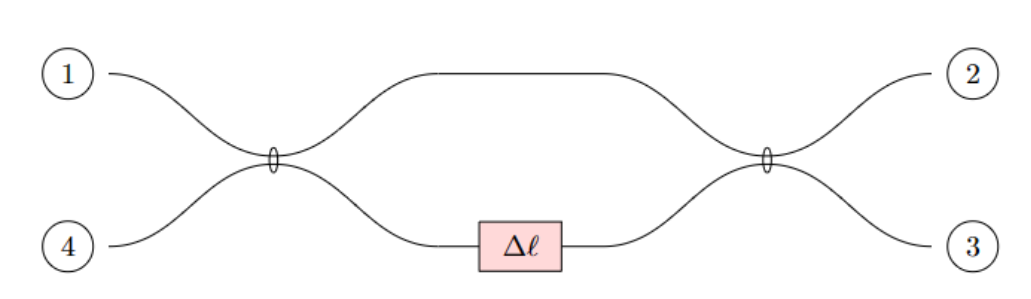
\includegraphics[width=0.4\textwidth]{figs/Mach-Zehnde.PNG}
\end{center}

\paragraph*{(a)} \textit{Using the reduced matrix of the directional coupler from the previous section, and a transfer matrix describing the propagation of the light in the two interferometer arms, write the matrix describing the whole system.} 

The reduced matrix of the directional coupler (basically, a beam splitter) is 
\begin{equation}
    S = \pmqty{
        -\alpha & \ii \beta \\
        \ii \beta & - \alpha
    },
\end{equation}
and therefore the matrix of the whole system is 
\begin{equation}
    \begin{aligned}
        S &= \pmqty{
            -\alpha & \ii \beta \\
            \ii \beta & - \alpha
        }^\dagger
        \pmqty{
            1 & \\
            & \ee^{\ii k \Delta l}
        }
        \pmqty{
            -\alpha & \ii \beta \\
            \ii \beta & - \alpha
        } \\
        &= \pmqty{
            \alpha^2 + \beta^2 \ee^{\ii k \Delta l} & 
            \ii \alpha \beta (-1 + \ee^{\ii k \Delta l}) \\
            \ii \alpha \beta (1 - \ee^{\ii k \Delta l}) & 
            \alpha^2 \ee^{\ii k \Delta l} + \beta^2
        }.
    \end{aligned}
\end{equation}

\paragraph*{(b)} \textit{Calculate the amplitude and phase response of the system, i.e. the scattering parameters $S_{21}$ and $S_{31}$ of the MZI. Show that energy is conserved.
[Note: This is an example of a finite impulse response (FIR) system, that has a transfer function with zeros, but no poles.]} 

The notation is slightly confusing:
$S_{21}$ means the matrix element of $1 \to 2$ and therefore is the $(1, 1)$ element of $S$, so 
\begin{equation}
    S_{21} = \alpha^2 + \beta^2 \ee^{\ii k \Delta l}, 
\end{equation} 
and similarly $S_{31}$ is the $(2, 1)$ element of $S$ and 
\begin{equation}
    S_{31} = \ii \alpha \beta (1 - \ee^{\ii k \Delta l}).
\end{equation}
To show energy conservation it's sufficient to show 
\begin{equation}
    \abs*{S_{21}}^2 + \abs*{S}_{31}^2 = 1,
\end{equation}
and since 
\[
    \abs*{S_{21}}^2 = \alpha^4 + \beta^4 + 2 \alpha^2 \beta^2 \cos k \Delta l,
\]
\[
    \abs*{S_{31}}^2 = \alpha^2 \beta^2 (2 - 2 \cos k \Delta l),
\]
we find 
\[
    \abs*{S_{21}}^2 + \abs*{S_{31}}^2 = (\alpha^2 + \beta^2)^2 = 1.
\]

\subsection{}

\textit{Two of the arms of a directional coupler can be connected to each other to form a ring of length $\ell$, such that the system has two ports, as shown below.}

\begin{center}
    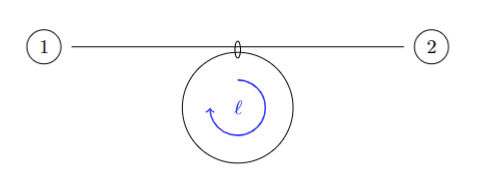
\includegraphics[width=0.4\textwidth]{figs/ring.PNG}
\end{center}

\paragraph*{(a)} \textit{Use the results obtained for the directional coupler to write the transfer matrix of a ring resonator. Write the amplitude and phase responses, and show that energy is conserved. (Hint: Since we are assuming no reflections, this reduces to a single parameter $S_{21}$ ).[Note: This is an example of an all-pass filter. It has both poles and zeros in its transfer function, that are arranges such that it does not affect the amplitude of the signal, however the phase of different spectral components is changed.]
} 

The equations are 
\begin{equation}
    \pmqty{a_1 \\ a_4} = \pmqty{- \alpha & \ii \beta \\ \ii \beta & - \alpha} \pmqty{a_2 \\ a_3},
\end{equation}
and 
\begin{equation}
    a_4 = \ee^{\ii k \Delta l} a_3.
\end{equation}
By eliminating $a_3$, we get 
\begin{equation}
    a_2 = - \frac{\alpha + \ee^{\ii k \Delta l}}{1 + \alpha \ee^{\ii k \Delta l}} a_1, \quad 
    a_3 = - \frac{\ii \beta}{1 + \alpha \ee^{\ii k \Delta l}}   .
\end{equation}
Therefore 
\begin{equation}
    S_{21} = - \frac{\alpha + \ee^{\ii k \Delta l}}{1 + \alpha \ee^{\ii k \Delta l}} ,
\end{equation}
and since 
\begin{equation}
    \abs*{S_{21}}^2 = \frac{\alpha^2 + 1 + 2 \cos k \Delta l}{1 + \alpha^2 + 2 \alpha \cos k \Delta l} = 1,
\end{equation}
the energy is conserved.

\paragraph*{(b)} \textit{Calculate the group delay $\tau_g$, and show how the input power times group delay is exactly equivalent to the energy stored in the ring resonator.} 

Suppose $\phi$ is the phase of $S_{21}$. 
Since the amplitude of $S_{21}$ is a constant, we have 
\[
    \dv{S_{21}}{\omega} = S_{21} \ii \dv{\phi}{\omega} ,
\]
and the group delay is 
\begin{equation}
    \tau_{\text{g}} = - \dv{\phi}{\omega} = \ii \frac{1}{S_{21}} \dv{S_{21}}{\omega}
    = \frac{\beta^2}{1 + \alpha^2 + 2 \alpha \cos k \Delta l} \frac{\Delta l}{c}.
\end{equation}

The energy stored in the ring resonator is 
\begin{equation}
    U_{\text{stored}} = \Delta l \abs*{a_3}^2 = \Delta l \frac{\beta^2}{1 + \alpha^2 + 2 \alpha \cos k \Delta l} \abs*{a_1}^2,
\end{equation}
and therefore 
\begin{equation}
    U_{\text{stored}} = \tau_{\text{g}} \cdot \abs*{a_1}^2 c = \tau_{\text{g}} \cdot P_{\text{input}}.
\end{equation}

\paragraph*{(c)} \textit{In practice, ring resonators are used as filters with a frequency-dependent output power. This is a consequence of the internal loss associated with propagation in the ring. Assuming the loss of a round trip in the ring is given by $\alpha$, calculate the ring response and find the free spectral range (FSR).} 

Now we need to solve 
\begin{equation}
    \pmqty{a_1 \\ a_4} = \pmqty{- \alpha & \ii \beta \\ \ii \beta & - \alpha} \pmqty{a_2 \\ a_3}, \quad 
    a_4 = \ee^{\ii k \Delta l} (1 - \gamma) a_3.
\end{equation}
Here $\gamma$ is used to refer to the loss, 
because $\alpha$ is already used to refer to $S_{11}$ of the beam splitter.
Then we get 
\begin{equation}
    a_3 = - \frac{\ii \beta}{1 + (1 - \gamma) \alpha \ee^{\ii k \Delta l}} a_1.
\end{equation}
The energy transfer is given by 
\begin{equation}
    S_{31} = \abs*{a_3 / a_1}^2 = \frac{\beta^2}{1 + (1 - \gamma)^2 \alpha^2 + 2 (1 - \gamma) \alpha \cos k \Delta l}.
\end{equation}
The FSR of frequency is $c \pi / \Delta l$.

\textit{We can alternatively use coupled mode theory to describe the ring resonator as a mode $(a)$ with wave amplitudes going in $\left(s^i\right)$ and out $\left(s^o\right)$ of the resonator, corresponding to the waves propagating into Port 1 and out of Port 2, respectively. The coupled mode equations we have derived in the lectures can be used for a uni-directional wave coupled to a mode, such as the ring resonator. The phase convention used to describe such a system can be different, as shown below (this is a consequence of choosing a different phase for $\gamma$ when deriving the coupled-mode equations, and is equivalent to changing a reference plane, as we saw for the scattering matrix earlier).}

\textit{(d)} \textit{Using temporal coupled mode theory, and assuming the mode has a resonant frequency $\omega_0$ and dissipation time $\tau$, write the measured output wave for a given input, i.e. $s^o / s^i$. You can assume no internal loss in the resonator in this case.} 

The EOMs are the simple 
\begin{equation}
    \dot{a} = - \ii \omega_0 a - \frac{1}{\tau} a + \sqrt{\frac{2}{\tau}} \Si{}, \quad 
    \So{} = - \Si{} + \sqrt{\frac{2}{\tau}} a.
\end{equation}
Repeating what is done above, in Fourier domain we have 
\[
    a(\omega) = \frac{1}{- \ii \omega + \ii \omega_0 + \frac{1}{\tau}} \sqrt{\frac{2}{\tau}} \Si{},
\]
and therefore 
\begin{equation}
    \frac{\So{}}{\Si{}} = - 1 + \frac{2}{\tau} \frac{1}{- \ii \omega + \ii \omega_0 + \frac{1}{\tau}} = 
    \frac{\ii \omega - \ii \omega_0 + \frac{1}{\tau}}{- \ii \omega + \ii \omega_0 + \frac{1}{\tau}}.
\end{equation}

\section{}

\textit{In this question, we will examine an important component in optical experiments, the beam splitter. Practically, beam splitters can be implemented using a partially-reflecting mirror, or a directional coupler, which can be a fiber-optical component, or an integrated photonic device, as illustrated below.}

\textit{We have already analyzed such devices in a classical framework in Question 2.2. However, when treating the beam splitter within the context of quantum-optics, the classical analysis leads to misleading results when considering non-classical states of light, and a full quantum analysis must be carried out. For a full quantum analysis, we replace the classical waves we have used to describe the modes with annihilation operators $\hat{a}_k$, where $k=\{1,2,3,4\}$ (see illustration).
Here, we will consider a beam splitter that equally splits power between the output ports (commonly referred to as a 50:50 splitter). As we have seen in Question 2.2, the matrix relating the output modes $\left(\hat{a}_3, \hat{a}_4\right)$ to the input waves $\left(\hat{a}_1, \hat{a}_2\right)$ is not uniquely defined, and for this question, we will choose the form}
$$
\left(\begin{array}{l}
\hat{a}_3 \\
\hat{a}_4
\end{array}\right)=\frac{1}{\sqrt{2}}\left(\begin{array}{ll}
1 & i \\
i & 1
\end{array}\right)\left(\begin{array}{l}
\hat{a}_1 \\
\hat{a}_2
\end{array}\right) .
$$

\textit{We know that the operators describing the input modes $\left(\hat{a}_1, \hat{a}_2\right)$ must obey Bosonic commutation relations, given by
$$
\left[\hat{a}_i, \hat{a}_j^{\dagger}\right]=\delta_{i j}, \quad\left[\hat{a}_i, \hat{a}_j\right]=\left[\hat{a}_i^{\dagger}, \hat{a}_j^{\dagger}\right]=0, \quad i, j=\{1,2\} .
$$
Show that the output modes $\left(\hat{a}_3, \hat{a}_4\right)$ also obey the Bosonic commutator relations.}

We can directly verify the commutation relations of $a_{3,4}$.
We have 
\begin{equation}
    \comm*{a_3}{a_4} = \frac{1}{2} \comm*{a_1 + \ii a_2}{\ii a_1 + a_2}
    = \frac{1}{2} (\comm*{a_1}{a_2} - \ii \comm*{a_2}{a_1}) = 0,
\end{equation}
and trivially $\comm*{a_3}{a_3} = \comm*{a_4}{a_4} = 0$.
Therefore $\comm*{a_i}{a_j} = 0$ is true for $a_{3,4}$, 
and hence we also have $\comm*{a_i^\dagger}{a_j^\dagger} = 0$.
Also, we have 
\begin{equation}
    \comm*{a_3}{a_3^\dagger} = \frac{1}{2} \comm*{a_1 + \ii a_2}{a_1^\dagger - \ii a_2^\dagger}
    = \frac{1}{2} \cdot 2 = 1, 
\end{equation}
and similarly 
\begin{equation}
    \comm*{a_4}{a_4^\dagger} = \frac{1}{2} \comm*{\ii a_1 + a_2}{- \ii a_1^\dagger + a_2^\dagger}
    = \frac{1}{2} \cdot 2 = 1,
\end{equation}
while 
\begin{equation}
    \comm*{a_3}{a_4^\dagger} = \frac{1}{2} \comm*{a_1 + \ii a_2}{- \ii a_1^\dagger + a_2^\dagger}
    = \frac{1}{2} \cdot (- \ii + \ii) = 0
\end{equation}
and hence $\comm*{a_4}{a_3^\dagger} = 0$.
So far we have verified all bosonic commutation relations of $a_{3,4}$.

\end{document}